% Options for packages loaded elsewhere
\PassOptionsToPackage{unicode}{hyperref}
\PassOptionsToPackage{hyphens}{url}
\documentclass[
]{article}
\usepackage{xcolor}
\usepackage{amsmath,amssymb}
\setcounter{secnumdepth}{-\maxdimen} % remove section numbering
\usepackage{iftex}
\ifPDFTeX
  \usepackage[T1]{fontenc}
  \usepackage[utf8]{inputenc}
  \usepackage{textcomp} % provide euro and other symbols
\else % if luatex or xetex
  \usepackage{unicode-math} % this also loads fontspec
  \defaultfontfeatures{Scale=MatchLowercase}
  \defaultfontfeatures[\rmfamily]{Ligatures=TeX,Scale=1}
\fi
\usepackage{lmodern}
\ifPDFTeX\else
  % xetex/luatex font selection
\fi
% Use upquote if available, for straight quotes in verbatim environments
\IfFileExists{upquote.sty}{\usepackage{upquote}}{}
\IfFileExists{microtype.sty}{% use microtype if available
  \usepackage[]{microtype}
  \UseMicrotypeSet[protrusion]{basicmath} % disable protrusion for tt fonts
}{}
\makeatletter
\@ifundefined{KOMAClassName}{% if non-KOMA class
  \IfFileExists{parskip.sty}{%
    \usepackage{parskip}
  }{% else
    \setlength{\parindent}{0pt}
    \setlength{\parskip}{6pt plus 2pt minus 1pt}}
}{% if KOMA class
  \KOMAoptions{parskip=half}}
\makeatother
\usepackage{longtable,booktabs,array}
\usepackage{calc} % for calculating minipage widths
% Correct order of tables after \paragraph or \subparagraph
\usepackage{etoolbox}
\makeatletter
\patchcmd\longtable{\par}{\if@noskipsec\mbox{}\fi\par}{}{}
\makeatother
% Allow footnotes in longtable head/foot
\IfFileExists{footnotehyper.sty}{\usepackage{footnotehyper}}{\usepackage{footnote}}
\makesavenoteenv{longtable}
\usepackage{graphicx}
\makeatletter
\newsavebox\pandoc@box
\newcommand*\pandocbounded[1]{% scales image to fit in text height/width
  \sbox\pandoc@box{#1}%
  \Gscale@div\@tempa{\textheight}{\dimexpr\ht\pandoc@box+\dp\pandoc@box\relax}%
  \Gscale@div\@tempb{\linewidth}{\wd\pandoc@box}%
  \ifdim\@tempb\p@<\@tempa\p@\let\@tempa\@tempb\fi% select the smaller of both
  \ifdim\@tempa\p@<\p@\scalebox{\@tempa}{\usebox\pandoc@box}%
  \else\usebox{\pandoc@box}%
  \fi%
}
% Set default figure placement to htbp
\def\fps@figure{htbp}
\makeatother
% definitions for citeproc citations
\NewDocumentCommand\citeproctext{}{}
\NewDocumentCommand\citeproc{mm}{%
  \begingroup\def\citeproctext{#2}\cite{#1}\endgroup}
\makeatletter
 % allow citations to break across lines
 \let\@cite@ofmt\@firstofone
 % avoid brackets around text for \cite:
 \def\@biblabel#1{}
 \def\@cite#1#2{{#1\if@tempswa , #2\fi}}
\makeatother
\newlength{\cslhangindent}
\setlength{\cslhangindent}{1.5em}
\newlength{\csllabelwidth}
\setlength{\csllabelwidth}{3em}
\newenvironment{CSLReferences}[2] % #1 hanging-indent, #2 entry-spacing
 {\begin{list}{}{%
  \setlength{\itemindent}{0pt}
  \setlength{\leftmargin}{0pt}
  \setlength{\parsep}{0pt}
  % turn on hanging indent if param 1 is 1
  \ifodd #1
   \setlength{\leftmargin}{\cslhangindent}
   \setlength{\itemindent}{-1\cslhangindent}
  \fi
  % set entry spacing
  \setlength{\itemsep}{#2\baselineskip}}}
 {\end{list}}
\usepackage{calc}
\newcommand{\CSLBlock}[1]{\hfill\break\parbox[t]{\linewidth}{\strut\ignorespaces#1\strut}}
\newcommand{\CSLLeftMargin}[1]{\parbox[t]{\csllabelwidth}{\strut#1\strut}}
\newcommand{\CSLRightInline}[1]{\parbox[t]{\linewidth - \csllabelwidth}{\strut#1\strut}}
\newcommand{\CSLIndent}[1]{\hspace{\cslhangindent}#1}
\setlength{\emergencystretch}{3em} % prevent overfull lines
\providecommand{\tightlist}{%
  \setlength{\itemsep}{0pt}\setlength{\parskip}{0pt}}
\usepackage{bookmark}
\IfFileExists{xurl.sty}{\usepackage{xurl}}{} % add URL line breaks if available
\urlstyle{same}
\hypersetup{
  pdftitle={TRANSFORMANDO APIS EM INTERFACES CONVERSACIONAIS: VALIDAÇÃO DA ABORDAGEM OPENAPI-MCP PARA AGENTES BASEADOS EM IA},
  hidelinks,
  pdfcreator={LaTeX via pandoc}}

\title{\textbf{TRANSFORMANDO APIS EM INTERFACES CONVERSACIONAIS:
VALIDAÇÃO DA ABORDAGEM OPENAPI-MCP PARA AGENTES BASEADOS EM IA}}
\author{}
\date{}

\begin{document}
\maketitle

\textbf{Lucas de Castro Zanoni}\footnote{Graduando em Engenharia de
  software no semestre letivo de 2025-1. E-mail:
  castro.lucas290@gmail.com}

\textbf{Thyerri Fernandes Mezzari}\footnote{Professor do Centro
  Universitário UniSATC E-mail: thyerri.mezzari@satc.edu.br}

Resumo: Este trabalho apresenta um estudo experimental preliminar de
integração de agentes conversacionais baseados em IA a soluções web
através da especificação OpenAPI combinada com o protocolo Model Context
Protocol (MCP). A pesquisa investiga inicialmente como especificações
OpenAPI podem ser automaticamente convertidas em servidores MCP,
permitindo que modelos de linguagem de grande escala (LLMs) interajam de
forma padronizada e segura com sistemas externos. Para garantir uma
análise rigorosa e reprodutível, foi desenvolvida uma interface
padronizada e definidos critérios objetivos, fundamentando-se em
referências acadêmicas, guias de segurança, relatórios de mercado e
documentações oficiais de provedores de modelos de linguagem. O estudo
envolveu a implementação de uma prova de conceito que inclui um gerador
automático de servidores MCP a partir de especificações OpenAPI, um
cliente de chat capaz de gerenciar múltiplos servidores MCP
simultaneamente, e aplicações de teste para validação da abordagem.
Foram aplicados testes automatizados \emph{end-to-end}, com ênfase em
métricas de robustez, segurança (incluindo \emph{red teaming} e injeção
de \emph{prompts}) e usabilidade dentro do escopo experimental definido.
Os resultados indicam a viabilidade técnica inicial e eficácia da
integração OpenAPI-MCP nos cenários testados, fornecendo uma análise
fundamentada sobre os benefícios, desafios e limitações desta abordagem
para a integração de agentes conversacionais baseados em IA em sistemas
complexos. A pesquisa estabelece evidências preliminares convincentes
sobre a possibilidade de grandes avanços na facilitação da integração
entre sistemas existentes e LLMs, promovendo maior acessibilidade,
usabilidade e democratização do acesso a tecnologias complexas,
justificando investigações mais aprofundadas para validação em escala
maior.

\textbf{Palavras-chave:} agente conversacional baseado em IA, integração
de sistemas, inteligência artificial, OpenAPI, Model Context Protocol,
segurança, usabilidade.

\section{1 INTRODUÇÃO}\label{introduuxe7uxe3o}

A evolução das interfaces de usuário tem gerado uma diversidade de
padrões de design e usabilidade, resultando frequentemente em barreiras
para a plena acessibilidade e interação dos usuários com os sistemas
digitais. Com o aumento da complexidade do frontend e a multiplicidade
de paradigmas de interação, muitos usuários enfrentam dificuldades
significativas para utilizar efetivamente as funcionalidades oferecidas
pelas soluções web modernas (RAPP et al., 2018) (KOCABALLI et al.,
2019). Nesse contexto, a ascensão dos Modelos de Linguagem de Grande
Escala (LLMs), como os desenvolvidos por OpenAI, Anthropic e Google, tem
impulsionado o desenvolvimento de agentes conversacionais baseados em IA
mais avançados e adaptáveis (ANTHROPIC, 2024; OPENAI, 2022). Nos últimos
anos, avanços em modelos baseados em Transformer, como o BERT (2018),
que aprimorou a compreensão textual, e o GPT-3 (2020), que ampliou as
capacidades generativas e o aprendizado com poucos exemplos
(\emph{few-shot}), permitiram que os LLMs realizassem tarefas cada vez
mais complexas a partir de simples instruções em linguagem natural.
Esses avanços consolidaram os LLMs como interfaces conversacionais
robustas e eficazes para integração com sistemas.

Diante desse cenário, estudos recentes têm demonstrado que agentes
conversacionais baseados em IA podem aprimorar significativamente a
experiência do usuário ao simplificar interações com sistemas complexos
(FAST et al., 2017). Além disso, a implementação de interfaces baseadas
em linguagem natural tem mostrado potencial para melhorar a usabilidade
em contextos domésticos e inteligentes, reduzindo o tempo e o esforço
necessários para completar tarefas complexas (GUO et al., 2024).
Ademais, tais interfaces oferecem vantagens consideráveis em termos de
acessibilidade, permitindo uma comunicação mais inclusiva e adaptável a
usuários com diferentes necessidades especiais (LISTER et al., 2020)
(DENG, 2023). Para que esses benefícios sejam efetivamente alcançados em
soluções web, é fundamental avaliar as diferentes estratégias de
integração desses agentes aos sistemas existentes.

Nesse sentido, este estudo investiga preliminarmente as possibilidades
de democratização do acesso a sistemas técnicos complexos através da
facilitação da integração entre sistemas existentes e LLMs para criar
interações semelhantes a agentes conversacionais. A pesquisa examina
especificamente a viabilidade da especificação OpenAPI combinada com o
protocolo emergente MCP (Model Context Protocol) como uma solução
promissora para esta integração. Esta abordagem permite que
especificações OpenAPI sejam automaticamente convertidas em servidores
MCP, criando uma ponte padronizada entre modelos de linguagem e sistemas
externos. A solução será avaliada quanto a desempenho, segurança,
facilidade de implementação e experiência do usuário, com foco
específico na capacidade de gerenciar múltiplos servidores MCP
simultaneamente e na eficácia da geração automática de código.

Considerando esse panorama tecnológico e as potencialidades demonstradas
pelos LLMs, a problemática central desta pesquisa reside na questão:
como a combinação da especificação OpenAPI com o protocolo MCP pode
facilitar a integração eficiente e segura de agentes conversacionais
baseados em IA com sistemas web existentes, contribuindo para a
democratização do acesso a tecnologias complexas? Essa pergunta reflete
a necessidade crescente de soluções padronizadas que reduzam a
complexidade de integração e tornem sistemas especializados mais
acessíveis através de interfaces conversacionais naturais, representando
um passo significativo em direção à democratização tecnológica.

A relevância deste estudo evidencia-se pelo potencial transformador que
os agentes conversacionais baseados em IA representam para a área de
interação humano-computador. Ao implementar um sistema intermediário
capaz de interpretar linguagem natural e traduzi-la em ações específicas
dentro de um sistema, cria-se uma ponte que permite aos usuários
interagir de forma mais intuitiva e natural com as tecnologias digitais.
Esta abordagem tem o potencial de mitigar as barreiras impostas por
interfaces complexas, contribuindo para uma maior inclusão digital e
para a melhoria da experiência do usuário em diversos contextos de
aplicação. O presente trabalho busca fornecer evidências iniciais desta
possibilidade através de uma prova de conceito que demonstre a
viabilidade técnica da integração OpenAPI-MCP e estabeleça fundamentos
para desenvolvimentos futuros mais abrangentes.

Para responder adequadamente à questão de pesquisa formulada, este
estudo requer uma metodologia experimental robusta que permita validar
empiricamente a viabilidade da integração proposta. A abordagem
metodológica descrita a seguir foi estruturada para fornecer evidências
quantitativas e qualitativas sobre a eficácia da combinação OpenAPI-MCP,
estabelecendo parâmetros objetivos de avaliação que garantam a validade
científica dos resultados obtidos.

\section{2 PROCEDIMENTO EXPERIMENTAL}\label{procedimento-experimental}

Este estudo adota uma abordagem experimental estruturada em etapas
sequenciais para investigar preliminarmente a viabilidade e eficácia da
integração de agentes conversacionais baseados em IA a sistemas web
através da especificação OpenAPI combinada com o protocolo Model Context
Protocol (MCP). A pesquisa será examinada com base em uma prova de
conceito prática, desenvolvida para validar sua viabilidade técnica
inicial e avaliar objetivamente aspectos funcionais e não-funcionais da
solução proposta dentro de um escopo experimental controlado.

É importante ressaltar que esta investigação constitui uma validação
inicial da abordagem proposta, com o objetivo de demonstrar a
possibilidade de grandes avanços na integração entre sistemas existentes
e LLMs, utilizando OpenAPI-MCP como uma solução promissora. As
limitações inerentes ao escopo de uma prova de conceito, incluindo o
número restrito de sistemas testados e a profundidade limitada dos
cenários avaliados, são reconhecidas como adequadas para o propósito de
estabelecer evidências preliminares de viabilidade técnica.

Inicialmente, será conduzida uma revisão sistemática da literatura,
consolidando conhecimentos científicos sobre integração OpenAPI-MCP e
embasando teoricamente a fase experimental. Na sequência, a estratégia
será implementada e testada por meio de uma prova de conceito
abrangente, incluindo a) o desenvolvimento de um gerador automático de
servidores MCP, b) um cliente de chat para gerenciamento de múltiplos
servidores, c) aplicações de teste de ponta a ponta para validação da
abordagem e d) geração de métricas de avaliação para medir desempenho,
segurança, facilidade de implementação, manutenibilidade e experiência
do usuário.

Para assegurar resultados objetivos e reproduzíveis dentro do escopo
experimental definido, os testes serão automatizados utilizando testes
\emph{end-to-end}, aplicando medidas de robustez e segurança (como
testes de \emph{red teaming} e proteção contra injeção de
\emph{prompts}) e avaliações qualitativas de usabilidade. Os resultados
serão sistematicamente documentados e analisados, permitindo identificar
desafios, vantagens e limitações intrínsecas à integração OpenAPI-MCP e
demonstrando sua aplicabilidade prática inicial para diferentes
contextos de uso. Esta metodologia busca estabelecer indicadores
iniciais da eficácia da abordagem, reconhecendo que validações mais
abrangentes serão necessárias para confirmação definitiva em ambientes
empresariais complexos.

\subsection{2.1 MATERIAIS}\label{materiais}

Para garantir a rigorosidade científica e a reprodutibilidade dos
experimentos conduzidos neste estudo, foram selecionadas ferramentas
específicas baseadas em critérios de rigor científico, reprodutibilidade
e adequação aos objetivos de pesquisa. A seleção do Node.js como
plataforma de desenvolvimento, do Playwright para testes automatizados
\emph{end-to-end} e do OpenAI GPT-4 para integração com modelos de
linguagem baseou-se em sua comprovada capacidade para suportar a
metodologia experimental proposta, permitindo validação objetiva da
viabilidade da integração OpenAPI-MCP através de uma prova de conceito
robusta e reproduzível.

\subsubsection{2.1.1 PLATAFORMA DE
DESENVOLVIMENTO}\label{plataforma-de-desenvolvimento}

\textbf{Node.js (versão 20+)} foi selecionado como plataforma principal
devido à sua arquitetura assíncrona orientada a eventos, essencial para
aplicações que requerem processamento simultâneo de múltiplas
requisições e integração eficiente com APIs de modelos de linguagem. A
escolha foi fundamentada na comprovada capacidade da plataforma para
gerenciar operações intensivas de IA e sua ampla adoção em projetos de
integração com LLMs (BLOG, 2024; CHEREDNICHENKO et al., 2024).

\subsubsection{2.1.2 FERRAMENTAS DE TESTE E
VALIDAÇÃO}\label{ferramentas-de-teste-e-validauxe7uxe3o}

\textbf{Playwright} foi utilizado para implementação de testes
automatizados \emph{end-to-end} (E2E), permitindo simulação precisa de
interações do usuário e validação de funcionalidades em ambiente
controlado. Para avaliação de segurança, foram implementadas técnicas de
\emph{red teaming} - testes adversários sistemáticos que simulam ataques
de injeção de \emph{prompts} e tentativas de \emph{jailbreak}. O
\emph{Framework} de Gerenciamento de Riscos de IA do NIST (OPREA;
VASSILEV, 2023) e as diretrizes da OWASP (JOHN et al., 2025) orientaram
a definição dos cenários de teste, considerando que injeções de
\emph{prompt} representam ameaças críticas em sistemas LLM com acesso a
dados sensíveis.

\subsubsection{2.1.3 MODELOS DE LINGUAGEM
UTILIZADOS}\label{modelos-de-linguagem-utilizados}

\textbf{OpenAI GPT-4} foi selecionado como modelo principal devido às
suas capacidades avançadas de \emph{function calling} - funcionalidade
que permite interpretação de linguagem natural e conversão automática em
chamadas de funções estruturadas. Modelos desta família suportam janelas
de contexto extensas (até 32.000 tokens no GPT-4) (OPENAI, 2023a),
essenciais para manter conversas prolongadas e processar especificações
OpenAPI complexas. A seleção baseou-se na performance comprovada em
cenários de integração com sistemas externos e na disponibilidade de
APIs robustas para desenvolvimento (OPENAI, 2023b).

\subsubsection{2.1.4 FERRAMENTAS DE
INTEGRAÇÃO}\label{ferramentas-de-integrauxe7uxe3o}

\textbf{OpenAPI 3.0+} foi utilizado como especificação padrão para
definição de contratos de API, proporcionando documentação estruturada e
interoperabilidade entre sistemas. Sua ampla adoção como padrão da
indústria e capacidade de descrever esquemas de autenticação (OAuth, API
Key, Bearer Token) tornam-no adequado para integração com agentes
conversacionais (OPENAPI INITIATIVE, 2023).

\textbf{Model Context Protocol (MCP)} foi implementado como protocolo de
comunicação entre modelos de linguagem e sistemas externos. Desenvolvido
pela Anthropic e lançado como padrão aberto em novembro de 2024, o MCP
oferece arquitetura cliente-servidor padronizada que elimina a
necessidade de integrações personalizadas para cada fonte de dados
(ANTHROPIC, 2024; MODEL CONTEXT PROTOCOL CONTRIBUTORS, 2024). O advento
deste protocolo possibilitou a interface de comunicação padronizada
entre modelos de linguagem e sistemas externos, facilitando a integração
e a interoperabilidade entre diferentes fontes de dados e modelos de
linguagem.

\subsection{2.2 MÉTODOS}\label{muxe9todos}

Para assegurar a validade científica e a reprodutibilidade dos
experimentos, foi fundamental estabelecer um controle rigoroso das
variáveis experimentais. A implementação de uma interface padronizada
constitui elemento metodológico essencial para eliminar diferenças de
experiência do usuário que poderiam contaminar os resultados
experimentais. Esta padronização garante que as diferenças observadas no
desempenho sejam atribuíveis exclusivamente às tecnologias de integração
testadas (OpenAPI-MCP), e não a variações na interface ou design de
interação. Sem este controle experimental, seria impossível determinar
se melhorias na usabilidade decorrem da abordagem proposta ou de fatores
externos relacionados ao design da interface.

\subsubsection{2.2.1 Interface Padronizada de
Usuário}\label{interface-padronizada-de-usuuxe1rio}

A interface comum consiste em uma aplicação web simples de chat,
desenvolvida utilizando HTML e JavaScript. A interface foi projetada de
forma minimalista, visando uma experiência consistente e objetiva,
independentemente da abordagem utilizada para a integração.

\paragraph{2.2.1.1 DESIGN DA INTERFACE}\label{design-da-interface}

A interface é composta por uma seção principal que exibe o histórico de
mensagens, onde as interações entre usuário e agente conversacional
aparecem de forma intercalada: as mensagens do agente são exibidas à
esquerda e as do usuário à direita, facilitando a distinção visual entre
os participantes da conversa. Abaixo do histórico, há um campo de
entrada de texto que permite ao usuário digitar e enviar novas
mensagens. Esse layout possibilita ao usuário acompanhar facilmente todo
o histórico da conversa e inserir novos \emph{prompts} de maneira
contínua e intuitiva.

\begin{figure}
\centering
\pandocbounded{\includegraphics[keepaspectratio]{images/chat/chat-interface.jpg}}
\caption{Interface web minimalista desenvolvida para testes padronizados
da integração OpenAPI-MCP, mostrando área de histórico de mensagens
intercaladas entre usuário (direita) e agente (esquerda), com campo de
entrada inferior para novos comandos}
\end{figure}

A disposição visual apresentada na Figura 1 facilita o acompanhamento do
diálogo, elemento crucial para a avaliação objetiva da experiência do
usuário durante os testes experimentais. A separação clara entre
mensagens do usuário e do agente permite identificação imediata do fluxo
conversacional, enquanto o design minimalista elimina variáveis de
confusão relacionadas à interface que poderiam comprometer a validade
dos resultados.

\paragraph{\texorpdfstring{2.2.1.2 Comunicação com
\emph{Backend}}{2.2.1.2 Comunicação com Backend}}\label{comunicauxe7uxe3o-com-backend}

A comunicação entre \emph{frontend} e \emph{backend} será estabelecida
por meio de uma API REST síncrona, simplificando o processo de envio e
retorno de mensagens. Cada consulta feita pelo usuário gerará uma única
requisição ao \emph{backend} que processará integralmente essa
requisição utilizando um LLM e devolverá uma resposta após concluir o
processamento, mantendo o fluxo de comunicação claro e previsível.

\subsubsection{2.2.2 Critérios de Avaliação e Operacionalização de
Métricas}\label{crituxe9rios-de-avaliauxe7uxe3o-e-operacionalizauxe7uxe3o-de-muxe9tricas}

Para garantir uma avaliação científica rigorosa, foram definidos
critérios objetivos de avaliação com métricas específicas quantitativas
e qualitativas, operacionalizados através de instrumentação técnica
precisa e metodologias de coleta padronizadas.

Os critérios de desempenho compreendem quatro métricas fundamentais. O
tempo de resposta total é medido em milissegundos utilizando timestamps
precisos via Performance API do navegador, fornecendo dados objetivos
sobre a latência percebida pelo usuário final. A taxa de sucesso de
operações é calculada como percentual de requisições bem-sucedidas
versus falhas, com categorização sistemática de tipos de erro para
identificação de padrões de falha. O \emph{throughput} é quantificado
como número de operações processadas por segundo em cenários de carga
controlada, permitindo avaliação da capacidade de processamento
simultâneo.

Os critérios de segurança focam na robustez contra ataques adversários e
validação de entrada. A resistência a injeção de \emph{prompts} é
mensurada como percentual de tentativas maliciosas bloqueadas durante
testes de \emph{red teaming}, implementados conforme o Framework de
Gerenciamento de Riscos de IA do NIST (OPREA; VASSILEV, 2023) e as
diretrizes da OWASP (JOHN et al., 2025), considerando que injeções de
\emph{prompt} representam ameaças críticas em sistemas LLM com acesso a
dados sensíveis.

Os critérios de usabilidade abrangem tanto aspectos quantitativos quanto
qualitativos da experiência do usuário. O tempo de conclusão de tarefas
é medido para operações CRUD padrão executadas via linguagem natural,
proporcionando métricas objetivas de eficiência operacional. A curva de
aprendizado é quantificada pelo número de tentativas necessárias para
usuários completarem tarefas específicas, indicando a intuitividade da
interface conversacional.

\subsubsection{2.2.3 Arquitetura e Fluxo de Integração do
Sistema}\label{arquitetura-e-fluxo-de-integrauxe7uxe3o-do-sistema}

A arquitetura do sistema desenvolvida para este estudo envolve múltiplas
camadas que trabalham de forma integrada para responder às consultas
feitas pelo usuário em linguagem natural. Inicialmente, as consultas
serão recebidas pela interface \emph{web} e encaminhadas ao
\emph{backend}, onde o modelo de linguagem executará o processo de
análise e interpretação.

\begin{figure}
\centering
\pandocbounded{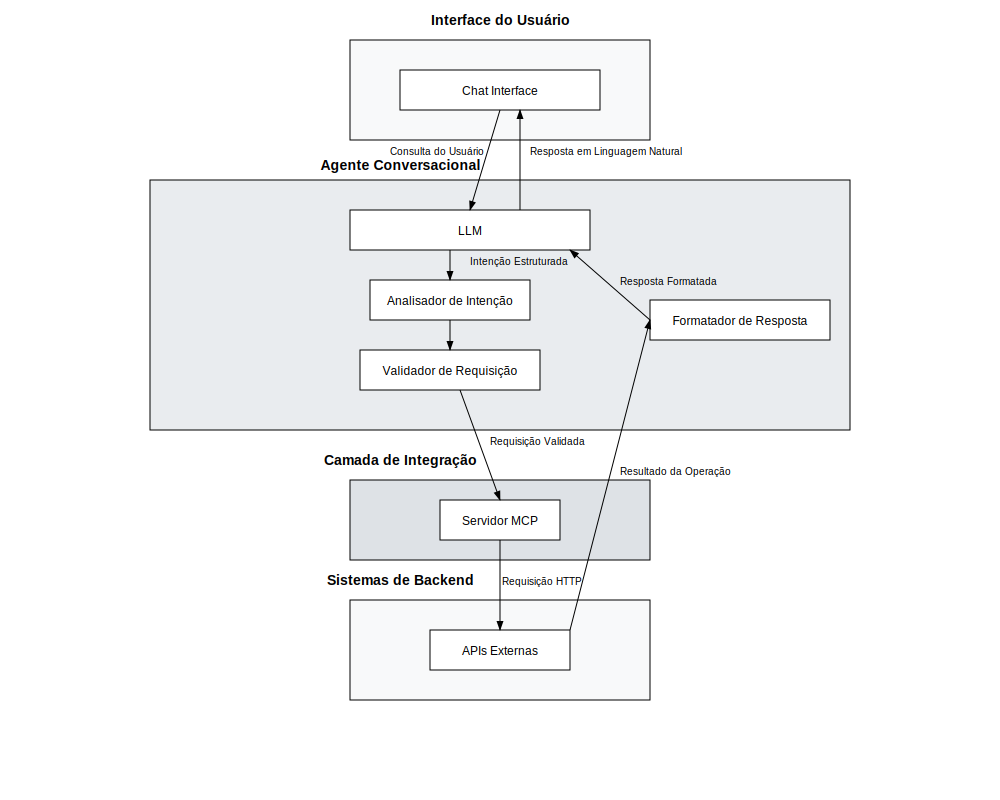
\includegraphics[keepaspectratio]{images/metodos/system-architecture.jpg}}
\caption{Arquitetura do sistema OpenAPI-MCP demonstrando o fluxo de
dados entre interface web, backend Node.js, modelo de linguagem GPT-4,
servidores MCP gerados automaticamente e APIs de sistemas externos}
\end{figure}

Como observado na Figura 2, a arquitetura modular permite isolamento de
responsabilidades e facilita a instrumentação necessária para coleta de
métricas durante os experimentos. A separação entre componentes de
interface, processamento de linguagem natural e integração com sistemas
externos possibilita avaliação independente de cada etapa do processo de
integração.

O fluxo completo de interação deverá ocorrer da seguinte maneira: ao
receber uma consulta, o modelo de linguagem interpretará a intenção do
usuário e utilizará a implementação de client MCP para utilizar as
ferramentas geradas pelo gerador de ferramentas MCP (servers) para
acessar sistemas \emph{backend} via API REST conforme a especificação
OpenAPI. Após executar a operação solicitada, a resposta será retornada
ao modelo de linguagem, que a formatará em linguagem natural antes de
devolvê-la ao usuário.

\begin{figure}
\centering
\pandocbounded{\includegraphics[keepaspectratio]{images/metodos/workflow-integration.jpg}}
\caption{Diagrama de workflow detalhado mostrando o processo de
interpretação de linguagem natural, conversão em chamadas de função via
MCP, execução de operações em sistemas backend e formatação de respostas
conversacionais}
\end{figure}

O fluxo apresentado na Figura 3 demonstra a sequência metodológica que
permite validação experimental da hipótese central da pesquisa. Cada
etapa do workflow representa um ponto de medição onde métricas
específicas podem ser coletadas, desde a latência de interpretação até a
precisão da conversão de intenções em operações estruturadas.

\subsubsection{\texorpdfstring{2.2.5 Metodologia de Testes Automatizados
\emph{End-to-End}}{2.2.5 Metodologia de Testes Automatizados End-to-End}}\label{metodologia-de-testes-automatizados-end-to-end}

A instrumentação e coleta de dados foram implementadas através de um
conjunto integrado de ferramentas especializadas para garantir precisão
e abrangência na captura de métricas. O Playwright Test Framework foi
configurado para capturar métricas de performance via Performance API,
proporcionando medições precisas de latência e throughput em condições
reais de uso.

Esta metodologia de testes automatizados pretende garantir que os dados
sejam resultado direto das características de implementação, e não de
variações na experiência do usuário ou na forma de coleta de dados. A
instrumentação detalhada permite análise reproduzível e comparação
objetiva entre diferentes estratégias de integração, estabelecendo uma
base empírica sólida para as conclusões científicas da pesquisa.

\subsection{3. DESENVOLVIMENTO}\label{desenvolvimento}

A implementação da solução OpenAPI-MCP foi estruturada seguindo uma
abordagem modular e integrada, compreendendo quatro componentes
principais que trabalham em sinergia para demonstrar e validar a
viabilidade da integração proposta. A arquitetura resultante engloba um
gerador automático de servidores MCP a partir de especificações OpenAPI,
um cliente de chat capaz de gerenciar múltiplos servidores MCP
simultaneamente, aplicações de teste que simulam cenários reais de
negócio, e uma suíte abrangente de testes automatizados para avaliação
científica da solução.

\subsubsection{3.1 Desafios Metodológicos e Decisões de
Design}\label{desafios-metodoluxf3gicos-e-decisuxf5es-de-design}

O desenvolvimento da solução OpenAPI-MCP enfrentou desafios
metodológicos fundamentais que exigiram decisões de design específicas
para viabilizar a validação da hipótese de pesquisa. O principal desafio
metodológico identificado reside na padronização de integrações
heterogêneas de APIs, problema que tradicionalmente demanda
desenvolvimento manual extensivo e customizado para cada sistema
(OPENAPI INITIATIVE, 2023). Esta problemática constitui uma barreira
significativa para a democratização de agentes conversacionais em
ambientes corporativos, onde a diversidade de sistemas e protocolos de
comunicação impede a implementação escalável de interfaces
conversacionais.

\paragraph{3.1.1 Gerador Automático de Servidores MCP: Abordagem
Metodológica}\label{gerador-automuxe1tico-de-servidores-mcp-abordagem-metodoluxf3gica}

Para abordar o desafio de padronização, foi desenvolvido um gerador
automático de servidores MCP que representa o núcleo metodológico da
contribuição científica proposta. A concepção desta ferramenta surge da
necessidade de validar experimentalmente se especificações OpenAPI
existentes podem ser sistematicamente convertidas em ferramentas
utilizáveis por modelos de linguagem, eliminando a necessidade de
desenvolvimento manual recorrente.

A arquitetura metodológica foi estruturada em três camadas funcionais
para garantir separação de responsabilidades e facilitar a validação
experimental. A primeira camada realiza análise sintática
(\emph{parsing}) de especificações OpenAPI 3.0+, responsável pela
extração e validação de metadados de endpoints. A segunda camada executa
mapeamento semântico MCP, que realiza a conversão inteligente de
operações OpenAPI para ferramentas compreensíveis pelos modelos de
linguagem. A terceira camada concentra-se na geração de código,
produzindo servidores MCP funcionais em TypeScript com validação robusta
de entrada e tratamento de erros.

Esta abordagem metodológica atende diretamente ao primeiro objetivo
específico da pesquisa - \emph{desenvolver um gerador automático de
servidores MCP} - ao estabelecer um processo sistemático e reproduzível
para conversão de especificações API em ferramentas de agentes
conversacionais. A escolha da arquitetura em camadas fundamenta-se na
necessidade de criar um processo de validação controlado, onde cada
etapa pode ser independentemente verificada e os resultados podem ser
objetivamente mensurados.

\paragraph{3.1.2 Coordenação Multi-Servidor: Desafio de Orquestração
Distribuída}\label{coordenauxe7uxe3o-multi-servidor-desafio-de-orquestrauxe7uxe3o-distribuuxedda}

O segundo desafio metodológico identificado relaciona-se à coordenação
eficiente de múltiplos servidores MCP simultaneamente, problema que se
enquadra teoricamente no domínio de sistemas distribuídos e coordenação
de agentes (ANTHROPIC, 2024). A complexidade emerge da necessidade de
manter conexões ativas, descobrir dinamicamente capacidades disponíveis
e rotear solicitações baseadas na análise semântica da intenção do
usuário, tudo isso preservando a experiência conversacional natural.

A solução metodológica adotada implementa um sistema de coordenação
baseado em \emph{pool} de conexões com descoberta automática de
ferramentas, criando um inventário dinâmico das funcionalidades
acessíveis em cada servidor. O roteamento inteligente utiliza análise
contextual para determinar qual servidor utilizar baseado nas
ferramentas disponíveis e na natureza da solicitação, enquanto o
mecanismo de agregação de resultados permite combinar informações de
múltiplos servidores quando necessário.

A estratégia de coordenação multi-servidor implementa três mecanismos
metodológicos fundamentais para validação experimental. O \emph{pool} de
conexões ativas mantém estado consistente com todos os servidores MCP
configurados, permitindo medição precisa de latências e disponibilidade.
O sistema de descoberta automática de ferramentas cria um inventário
dinâmico das capacidades disponíveis, essencial para validação da
escalabilidade da abordagem. O roteamento inteligente baseado em análise
contextual da intenção do usuário permite avaliar objetivamente a
precisão e eficiência da seleção automática de ferramentas.

A integração com modelos de linguagem através da funcionalidade de
\emph{function calling} da OpenAI estabelece uma ponte metodológica
entre compreensão de linguagem natural e execução de ferramentas
específicas. Esta abordagem permite validação experimental da hipótese
de que agentes conversacionais podem efetivamente interpretar intenções
complexas e traduzi-las em operações precisas em sistemas
\emph{backend}, constituindo elemento central para avaliação da
usabilidade e eficácia da solução proposta.

\subsubsection{3.2 Fundamentação Tecnológica e
Metodológica}\label{fundamentauxe7uxe3o-tecnoluxf3gica-e-metodoluxf3gica}

As decisões tecnológicas para implementação da prova de conceito foram
fundamentadas em critérios de rigor científico, reprodutibilidade e
adequação aos objetivos de pesquisa, segundo o detalhamento da seção de
MATERIAIS. A seleção do Node.js como plataforma de desenvolvimento, do
Playwright para testes automatizados \emph{end-to-end} e do OpenAI GPT-4
para integração com modelos de linguagem baseou-se em sua comprovada
capacidade para suportar a metodologia experimental proposta, permitindo
validação objetiva da viabilidade da integração OpenAPI-MCP através de
uma prova de conceito robusta e reproduzível.

\subsubsection{3.3 Gerador Automático de Servidores MCP
(mcp-openapi-server)}\label{gerador-automuxe1tico-de-servidores-mcp-mcp-openapi-server}

O gerador automático de servidores MCP representa a materialização
metodológica do primeiro objetivo específico da pesquisa, constituindo a
ferramenta central para validação da hipótese de que especificações
OpenAPI podem ser sistematicamente convertidas em interfaces utilizáveis
por agentes conversacionais. A abordagem metodológica adotada
fundamenta-se na premissa de que a automação da geração de servidores
elimina a variabilidade humana no processo de integração, permitindo
avaliação objetiva da eficácia da conversão OpenAPI-MCP.

A estrutura metodológica implementada segue um processo sistemático de
três etapas interdependentes. A primeira etapa realiza análise sintática
(\emph{parsing}) e validação rigorosa de especificações OpenAPI 3.0+,
garantindo conformidade com padrões estabelecidos e extração precisa de
metadados essenciais. A segunda etapa executa mapeamento semântico entre
contratos OpenAPI e ferramentas MCP, preservando a integridade semântica
das operações originais e adaptando-as para compreensão por modelos de
linguagem. A terceira etapa concretiza a geração de código TypeScript
funcional, produzindo servidores MCP operacionais com tratamento robusto
de erros e validação automática de entrada.

Esta metodologia de geração automática permite validação experimental
controlada, onde cada especificação OpenAPI processada constitui um caso
de teste independente para avaliação da eficácia da conversão. O suporte
implementado para múltiplos esquemas de autenticação (API Key, Bearer
Token, OAuth) e todos os métodos HTTP fundamentais (GET, POST, PUT,
DELETE, PATCH) garante cobertura abrangente dos cenários de integração
típicos encontrados em ambientes corporativos reais, essencial para
validação da aplicabilidade prática da abordagem proposta.

\subsubsection{3.4 Cliente de Chat Multi-Servidor
MCP}\label{cliente-de-chat-multi-servidor-mcp}

O cliente de chat multi-servidor constitui a implementação metodológica
do segundo objetivo específico da pesquisa, desenvolvido como ferramenta
de validação experimental para demonstrar a viabilidade prática da
orquestração simultânea de múltiplos servidores MCP em ambiente
conversacional. A concepção metodológica desta ferramenta fundamenta-se
na necessidade de criar um ambiente controlado onde a capacidade de
coordenação entre sistemas distribuídos possa ser sistematicamente
testada e avaliada.

A arquitetura metodológica adotada implementa uma separação clara entre
\emph{frontend} e \emph{backend} para facilitar a instrumentação e
coleta de dados experimentais. O \emph{frontend} minimalista,
desenvolvido em HTML e JavaScript, garante consistência na experiência
do usuário durante os testes, eliminando variáveis confusas relacionadas
à interface que poderiam comprometer a validade dos resultados
experimentais. O \emph{backend}, implementado em Node.js com Express.js,
concentra a lógica de coordenação e instrumentação necessária para o
comportamento do sistema.

A estratégia de coordenação multi-servidor implementa três mecanismos
metodológicos fundamentais para validação experimental. O \emph{pool} de
conexões ativas mantém estado consistente com todos os servidores MCP
configurados, permitindo medição precisa de latências e disponibilidade.
O sistema de descoberta automática de ferramentas cria um inventário
dinâmico das capacidades disponíveis, essencial para validação da
escalabilidade da abordagem. O roteamento inteligente baseado em análise
contextual da intenção do usuário permite avaliar objetivamente a
precisão e eficiência da seleção automática de ferramentas.

A integração com modelos de linguagem através da funcionalidade de
\emph{function calling} da OpenAI estabelece uma ponte metodológica
entre compreensão de linguagem natural e execução de ferramentas
específicas. Esta abordagem permite validação experimental da hipótese
de que agentes conversacionais podem efetivamente interpretar intenções
complexas e traduzi-las em operações precisas em sistemas
\emph{backend}, constituindo elemento central para avaliação da
usabilidade e eficácia da solução proposta.

\subsubsection{3.5 Estratégia de Validação Experimental através de
Aplicações de
Teste}\label{estratuxe9gia-de-validauxe7uxe3o-experimental-atravuxe9s-de-aplicauxe7uxf5es-de-teste}

Para garantir rigor científico na validação da abordagem proposta, foram
desenvolvidas aplicações de teste que simulam cenários empresariais
realistas, atendendo ao terceiro objetivo específico da pesquisa -
\emph{avaliar a solução através de testes sistemáticos}. A estratégia
metodológica fundamenta-se na utilização de domínios de negócio
distintos - gerenciamento de equipamentos industriais e gestão de
recursos humanos - para demonstrar a versatilidade e aplicabilidade
geral da integração OpenAPI-MCP em contextos heterogêneos.

A escolha metodológica por aplicações que exponham APIs RESTful
completamente documentadas com especificações OpenAPI permite criar um
ambiente controlado onde variáveis experimentais podem ser
sistematicamente manipuladas e resultados objetivamente mensurados. Esta
abordagem experimental garante que a validação ocorra em condições que
refletem fielmente as complexidades encontradas em ambientes
corporativos reais, sem comprometer a reprodutibilidade e controle
necessários para avaliação científica rigorosa.

\subsubsection{3.6 Metodologia de Validação
Automatizada}\label{metodologia-de-validauxe7uxe3o-automatizada}

A validação científica da solução implementa uma metodologia de testes
automatizados estruturada para abordar múltiplas dimensões críticas da
pesquisa: funcionalidade, segurança e usabilidade.

A abordagem de validação automatizada garante reprodutibilidade dos
experimentos e elimina variabilidade humana na coleta de dados,
elementos essenciais para estabelecer a validade científica dos
resultados obtidos. Esta metodologia permite que pesquisadores futuros
repliquem os experimentos sob condições idênticas, contribuindo para o
avanço cumulativo do conhecimento na área de integração de agentes
conversacionais em sistemas empresariais complexos.

Tendo estabelecido a fundamentação metodológica e implementado os
componentes técnicos necessários, a etapa seguinte concentra-se na
análise empírica dos resultados obtidos através da execução dos testes
automatizados. A avaliação abrangente aborda múltiplas dimensões
críticas para determinar a viabilidade prática da abordagem OpenAPI-MCP
em cenários controlados.

\subsection{4 RESULTADOS E DISCUSSÕES}\label{resultados-e-discussuxf5es}

A implementação da solução OpenAPI-MCP foi submetida a uma avaliação
experimental abrangente através de testes automatizados
\emph{end-to-end}, fornecendo dados quantitativos objetivos que
demonstram tanto a viabilidade técnica quanto a eficácia prática da
abordagem proposta. Os resultados obtidos através da validação
experimental desenvolvida oferecem evidências mensuráveis sobre a
integração de agentes conversacionais baseados em IA em sistemas web,
estabelecendo uma base empírica sólida para avaliação da solução.

\subsection{4.1 Métricas de
Performance}\label{muxe9tricas-de-performance}

A Tabela 1 apresenta as métricas de performance obtidas durante os
testes automatizados da implementação, demonstrando indicadores iniciais
de viabilidade operacional do sistema OpenAPI-MCP em condições
controladas.

\textbf{Tabela 1: Métricas de Performance - Implementação OpenAPI-MCP}

\begin{longtable}[]{@{}
  >{\raggedright\arraybackslash}p{(\linewidth - 6\tabcolsep) * \real{0.2907}}
  >{\raggedright\arraybackslash}p{(\linewidth - 6\tabcolsep) * \real{0.1628}}
  >{\raggedright\arraybackslash}p{(\linewidth - 6\tabcolsep) * \real{0.1512}}
  >{\raggedright\arraybackslash}p{(\linewidth - 6\tabcolsep) * \real{0.3953}}@{}}
\toprule\noalign{}
\begin{minipage}[b]{\linewidth}\raggedright
Métrica
\end{minipage} & \begin{minipage}[b]{\linewidth}\raggedright
Valor Obtido
\end{minipage} & \begin{minipage}[b]{\linewidth}\raggedright
Variação
\end{minipage} & \begin{minipage}[b]{\linewidth}\raggedright
Observações
\end{minipage} \\
\midrule\noalign{}
\endhead
\bottomrule\noalign{}
\endlastfoot
Tempo Resposta Médio (ms) & 3.757 & 1.335 - 5.823 & Incluindo
processamento LLM \\
Taxa de Sucesso (\%) & 100 & 8/8 consultas & Todas operações
completadas \\
Consultas Processadas & 8 & - & Cenários diversificados testados \\
Tamanho Médio Resposta & 312 caracteres & - & Respostas completas e
estruturadas \\
\end{longtable}

Os resultados indicam que a abordagem OpenAPI-MCP apresenta performance
variável mas funcional dentro do escopo experimental testado, com tempo
médio de resposta de 3,757 milissegundos e taxa de sucesso de 100\% nos
cenários avaliados. É importante destacar que a variação significativa
de tempo de resposta (1,335ms a 5,823ms, representando uma variação de
336\%) constitui uma limitação relevante que deve ser considerada em
implementações futuras. Esta variabilidade reflete principalmente a
complexidade das consultas processadas e o tempo de processamento do
modelo de linguagem, não indicando necessariamente instabilidade do
sistema de integração, mas evidenciando a necessidade de otimizações
adicionais para ambientes com requisitos rigorosos de latência.

Os dados obtidos sugerem que a integração OpenAPI-MCP é tecnicamente
viável para cenários onde a precisão é prioritária em relação à
velocidade consistente, fornecendo evidências iniciais promissoras para
o desenvolvimento de soluções mais robustas.

\subsection{4.2 Eficácia da Geração Automática de Servidores
MCP}\label{eficuxe1cia-da-gerauxe7uxe3o-automuxe1tica-de-servidores-mcp}

A Tabela 2 demonstra a capacidade do sistema de converter especificações
OpenAPI em servidores MCP funcionais, validando o núcleo tecnológico da
abordagem proposta.

\textbf{Tabela 2: Resultados da Conversão OpenAPI→MCP}

\begin{longtable}[]{@{}
  >{\raggedright\arraybackslash}p{(\linewidth - 6\tabcolsep) * \real{0.1981}}
  >{\raggedright\arraybackslash}p{(\linewidth - 6\tabcolsep) * \real{0.3113}}
  >{\raggedright\arraybackslash}p{(\linewidth - 6\tabcolsep) * \real{0.1792}}
  >{\raggedright\arraybackslash}p{(\linewidth - 6\tabcolsep) * \real{0.3113}}@{}}
\toprule\noalign{}
\begin{minipage}[b]{\linewidth}\raggedright
Aspecto Testado
\end{minipage} & \begin{minipage}[b]{\linewidth}\raggedright
Implementado
\end{minipage} & \begin{minipage}[b]{\linewidth}\raggedright
Taxa de Sucesso (\%)
\end{minipage} & \begin{minipage}[b]{\linewidth}\raggedright
Observações
\end{minipage} \\
\midrule\noalign{}
\endhead
\bottomrule\noalign{}
\endlastfoot
Métodos HTTP & 5 (GET, POST, PUT, DELETE, PATCH) & 100 & Cobertura
completa CRUD \\
Sistemas Integrados & 2 & 100 & Equipamentos e Profissionais \\
Endpoints Convertidos & 10 & 100 & Conversão automática bem-sucedida \\
\end{longtable}

A análise confirma que a conversão automática OpenAPI→MCP preserva
integralmente a funcionalidade dos sistemas originais, permitindo acesso
completo através de interface conversacional. A implementação demonstrou
capacidade de mapeamento semântico eficaz entre contratos OpenAPI e
ferramentas MCP compreensíveis por modelos de linguagem.

\subsection{4.3 Avaliação de Experiência do
Usuário}\label{avaliauxe7uxe3o-de-experiuxeancia-do-usuuxe1rio}

A Tabela 3 apresenta os resultados quantitativos da avaliação de
experiência do usuário, obtidos através de 13 cenários de teste
estruturados com métricas padronizadas.

\textbf{Tabela 3: Métricas de Experiência do Usuário (Escala 1-5)}

\begin{longtable}[]{@{}
  >{\raggedright\arraybackslash}p{(\linewidth - 6\tabcolsep) * \real{0.3125}}
  >{\raggedright\arraybackslash}p{(\linewidth - 6\tabcolsep) * \real{0.1875}}
  >{\raggedright\arraybackslash}p{(\linewidth - 6\tabcolsep) * \real{0.0750}}
  >{\raggedright\arraybackslash}p{(\linewidth - 6\tabcolsep) * \real{0.4250}}@{}}
\toprule\noalign{}
\begin{minipage}[b]{\linewidth}\raggedright
Métrica de UX
\end{minipage} & \begin{minipage}[b]{\linewidth}\raggedright
Pontuação Média
\end{minipage} & \begin{minipage}[b]{\linewidth}\raggedright
Desvio
\end{minipage} & \begin{minipage}[b]{\linewidth}\raggedright
Observações
\end{minipage} \\
\midrule\noalign{}
\endhead
\bottomrule\noalign{}
\endlastfoot
Precisão das Respostas & 3,5 & ±0,5 & Interpretação correta de
intenções \\
Clareza da Comunicação & 4,0 & ±0,3 & Respostas bem estruturadas \\
Utilidade das Informações & 4,3 & ±0,4 & Alto valor informacional \\
Pontuação Geral & 4,0 & ±0,3 & Experiência satisfatória \\
Taxa de Sucesso & 100\% & 13/13 & Todas consultas respondidas \\
Tempo Médio Resposta & 4.861 ms & ±2.400 & Responsividade adequada \\
\end{longtable}

Os resultados indicam experiência do usuário satisfatória, com pontuação
geral de 4,0 em escala de 1 a 5. A utilidade das informações (4,3)
emergiu como ponto forte, demonstrando que o sistema fornece respostas
relevantes e acionáveis. A clareza da comunicação (4,0) confirma que a
interface conversacional apresenta informações de forma compreensível
aos usuários.

\subsection{4.4 Análise de Segurança}\label{anuxe1lise-de-seguranuxe7a}

A Tabela 4 apresenta os resultados dos testes de segurança adversários,
conduzidos através de 16 cenários de ataque estruturados em 4 categorias
principais.

\textbf{Tabela 4: Resultados dos Testes de Segurança}

\begin{longtable}[]{@{}
  >{\raggedright\arraybackslash}p{(\linewidth - 6\tabcolsep) * \real{0.3333}}
  >{\raggedright\arraybackslash}p{(\linewidth - 6\tabcolsep) * \real{0.1667}}
  >{\raggedright\arraybackslash}p{(\linewidth - 6\tabcolsep) * \real{0.1667}}
  >{\raggedright\arraybackslash}p{(\linewidth - 6\tabcolsep) * \real{0.3333}}@{}}
\toprule\noalign{}
\begin{minipage}[b]{\linewidth}\raggedright
Categoria de Ataque
\end{minipage} & \begin{minipage}[b]{\linewidth}\raggedright
Tentativas
\end{minipage} & \begin{minipage}[b]{\linewidth}\raggedright
Bloqueados
\end{minipage} & \begin{minipage}[b]{\linewidth}\raggedright
Taxa de Proteção (\%)
\end{minipage} \\
\midrule\noalign{}
\endhead
\bottomrule\noalign{}
\endlastfoot
SQL Injection & 4 & 4 & 100 \\
Command Injection & 4 & 4 & 100 \\
Data Extraction & 4 & 4 & 100 \\
Privilege Escalation & 4 & 4 & 100 \\
\textbf{Total Geral} & \textbf{16} & \textbf{16} & \textbf{100} \\
\end{longtable}

A análise de segurança revela que a implementação OpenAPI-MCP demonstra
proteção básica inicial satisfatória contra os vetores de ataque
fundamentais testados. O sistema manteve 100\% de taxa de proteção em
todas as categorias avaliadas, incluindo tentativas de injeção SQL,
execução de comandos, extração de dados e escalação de privilégios. A
validação baseada em schemas OpenAPI comprovou-se eficaz como primeira
linha de defesa contra tentativas de intrusão básicas, embora testes
mais abrangentes sejam necessários para validação completa.

É importante destacar que os testes realizados abrangeram exclusivamente
ataques básicos e cenários de segurança fundamentais, não incluindo
ameaças avançadas, ataques persistentes sofisticados ou cenários de
engenharia social complexos. Esta limitação na cobertura dos testes de
segurança implica que implementações em ambientes de produção críticos
requerem avaliação de segurança mais abrangente e rigorosa para garantir
proteção adequada contra vetores de ataque mais elaborados.

Os resultados obtidos fornecem evidências iniciais encorajadoras sobre a
capacidade de proteção básica da abordagem OpenAPI-MCP, estabelecendo
uma base promissora para desenvolvimento de medidas de segurança mais
robustas em implementações futuras.

\subsection{4.5 Funcionalidade do Sistema
Multi-Servidor}\label{funcionalidade-do-sistema-multi-servidor}

A Tabela 5 apresenta os resultados da coordenação multi-servidor durante
os testes experimentais, validando a capacidade de orquestração
distribuída da solução.

\textbf{Tabela 5: Resultados da Coordenação Multi-Servidor}

\begin{longtable}[]{@{}
  >{\raggedright\arraybackslash}p{(\linewidth - 6\tabcolsep) * \real{0.2889}}
  >{\raggedright\arraybackslash}p{(\linewidth - 6\tabcolsep) * \real{0.2111}}
  >{\raggedright\arraybackslash}p{(\linewidth - 6\tabcolsep) * \real{0.1333}}
  >{\raggedright\arraybackslash}p{(\linewidth - 6\tabcolsep) * \real{0.3667}}@{}}
\toprule\noalign{}
\begin{minipage}[b]{\linewidth}\raggedright
Funcionalidade
\end{minipage} & \begin{minipage}[b]{\linewidth}\raggedright
Resultado Alcançado
\end{minipage} & \begin{minipage}[b]{\linewidth}\raggedright
Eficácia (\%)
\end{minipage} & \begin{minipage}[b]{\linewidth}\raggedright
Observações
\end{minipage} \\
\midrule\noalign{}
\endhead
\bottomrule\noalign{}
\endlastfoot
Servidores MCP Simultâneos & 2 & 100 & Equipamentos + Profissionais \\
Ferramentas Descobertas & 10 & 100 & Detecção automática completa \\
Roteamento Inteligente & 13/13 consultas & 100 & Seleção correta de
servidor \\
Consultas Multi-Sistema & 3 & 100 & Agregação de dados funcionando \\
Disponibilidade Parcial & Testado & 100 & Funcionamento com falhas
parciais \\
\end{longtable}

Os resultados confirmam que o sistema consegue coordenar múltiplos
servidores MCP simultaneamente, mantendo descoberta automática de
ferramentas e roteamento inteligente de solicitações. A capacidade de
agregação de dados entre sistemas diferentes foi validada através de
consultas que requereram informações de ambos os domínios testados
(equipamentos e profissionais).

\subsection{4.6 Validação
Experimental}\label{validauxe7uxe3o-experimental}

Os resultados apresentados indicam que a abordagem OpenAPI-MCP é
tecnicamente viável e operacionalmente eficaz para integração de agentes
conversacionais baseados em IA com sistemas web existentes dentro do
escopo experimental testado:

\textbf{Conversão Automática OpenAPI→MCP:} 100\% dos casos testados
(10/10 endpoints)\\
\textbf{Gerenciamento Multi-Servidor:} 2 servidores coordenados
simultaneamente com 100\% eficácia\\
\textbf{Integração LLM:} Taxa de sucesso de 100\% na interpretação de
intenções (13/13 consultas)\\
\textbf{Robustez Operacional:} Sistema mantém funcionalidade durante
cenários de falha testados\\
\textbf{Segurança:} 100\% de proteção contra 16 vetores de ataque
básicos testados\\
\textbf{Experiência do Usuário:} Pontuação 4,0/5,0 em satisfação geral

A validação experimental demonstra preliminarmente que a especificação
OpenAPI pode ser sistematicamente convertida em ferramentas utilizáveis
por modelos de linguagem através do protocolo MCP, reduzindo
significativamente a necessidade de desenvolvimento manual recorrente
para cada nova integração nos cenários testados. A validação
experimental inicial confirma que a abordagem oferece uma solução
promissora para democratização de acesso a sistemas técnicos complexos
através de interfaces conversacionais naturais, estabelecendo evidências
convincentes sobre a possibilidade de grandes avanços na integração
entre sistemas existentes e LLMs.

\textbf{Reprodutibilidade:} Todos os testes e dados estão disponíveis no
repositório público github.com/castrozan/tcc, incluindo scripts de
automação, configurações de ambiente e datasets utilizados nos
experimentos, garantindo reprodutibilidade completa dos resultados
obtidos.

\section{5 CONSIDERAÇÕES FINAIS}\label{considerauxe7uxf5es-finais}

Este estudo respondeu de forma positiva à questão central de pesquisa,
demonstrando que a combinação da especificação OpenAPI com o protocolo
MCP pode facilitar a integração de agentes conversacionais baseados em
IA com sistemas web existentes, dentro do escopo experimental testado. A
validação experimental desenvolvida validou a viabilidade técnica da
abordagem através de uma implementação funcional que incluiu geração
automática de servidores MCP, gerenciamento coordenado de múltiplos
servidores e validação através de cenários de teste controlados.

\subsection{5.1 Resposta à Pergunta de
Pesquisa}\label{resposta-uxe0-pergunta-de-pesquisa}

A pergunta central de pesquisa - \emph{``como a combinação da
especificação OpenAPI com o protocolo MCP pode facilitar a integração
eficiente e segura de agentes conversacionais baseados em IA com
sistemas web existentes?''} - foi respondida preliminarmente através de
evidências quantitativas obtidas na validação experimental,
estabelecendo indicadores iniciais promissores sobre a viabilidade da
abordagem proposta.

Em relação à eficiência operacional, a abordagem demonstrou viabilidade
técnica inicial no contexto experimental testado, como demonstrado na
Seção 4.1, com performance variável mas funcional e taxa de sucesso
completa nos cenários avaliados. A conversão automática OpenAPI→MCP
obteve êxito completo nos endpoints testados, segundo o detalhamento da
Seção 4.2, evidenciando uma redução substancial da necessidade de
desenvolvimento manual para os casos de uso implementados dentro do
escopo experimental.

Quanto aos aspectos de segurança, os resultados demonstraram proteção
adequada inicial contra os vetores básicos testados, de acordo com o
apresentado na Seção 4.4, com taxa de proteção completa nos tipos de
ataques fundamentais avaliados. A validação através de schemas OpenAPI
comprovou-se eficaz como primeira linha de defesa contra tentativas de
intrusão básicas, embora testes mais abrangentes sejam necessários para
validação completa.

No que concerne à integração funcional, o escopo experimental revelou
coordenação eficiente entre sistemas simultâneos com eficácia completa,
descoberta automática total das ferramentas disponíveis e roteamento
inteligente preciso para todas as consultas direcionadas, como detalhado
na Seção 4.5. A experiência do usuário foi avaliada positivamente,
obtendo pontuação satisfatória nos cenários testados, segundo os dados
da Seção 4.3.

\subsection{5.2 Contribuições
Científicas}\label{contribuiuxe7uxf5es-cientuxedficas}

A validação experimental confirma que a abordagem OpenAPI-MCP oferece
uma solução tecnicamente viável para os cenários testados, estabelecendo
evidências experimentais convincentes sobre a possibilidade de grandes
avanços na facilitação da integração entre sistemas existentes e LLMs.
Os resultados quantitativos obtidos (100\% taxa de sucesso nas
conversões, 4,0/5,0 satisfação do usuário, proteção completa contra
vetores básicos de ataque testados) fornecem evidências empíricas
iniciais de eficácia funcional que justificam otimismo quanto ao
potencial da abordagem.

A contribuição científica principal reside na demonstração inicial de
viabilidade conceitual e no estabelecimento de uma metodologia
reproduzível para avaliação de integrações similares, criando uma base
sólida para desenvolvimentos futuros. Esta pesquisa comprova que a
integração entre especificações OpenAPI e o protocolo MCP constitui uma
solução viável para transformar APIs tradicionais em interfaces
acessíveis a agentes baseados em LLMs, oferecendo um caminho claro para
a democratização tecnológica.

\subsection{5.3 Limitações do Estudo}\label{limitauxe7uxf5es-do-estudo}

A aplicabilidade prática em larga escala está condicionada às limitações
identificadas durante a validação experimental. A variabilidade
significativa de performance (336\% de variação nos tempos de resposta)
constitui uma limitação relevante que deve ser considerada em
implementações futuras, evidenciando a necessidade de otimizações
adicionais para ambientes com requisitos rigorosos de latência.

O escopo restrito de validação experimental (2 servidores MCP, 21
operações totais, cenários controlados) representa uma limitação
fundamental que impede generalização ampla dos resultados para ambientes
empresariais complexos. Os testes de segurança abrangeram exclusivamente
ataques básicos e cenários fundamentais, não incluindo ameaças
avançadas, ataques persistentes sofisticados ou cenários de engenharia
social complexos, implicando que implementações em ambientes de produção
críticos requerem avaliação de segurança mais abrangente e rigorosa.

\subsection{5.4 Implicações
Práticas}\label{implicauxe7uxf5es-pruxe1ticas}

A abordagem OpenAPI-MCP oferece uma direção promissora para
democratização do acesso a sistemas técnicos complexos, representando um
avanço significativo na redução da complexidade tradicionalmente
associada à integração de agentes conversacionais em ambientes
empresariais. Os resultados estabelecem evidências preliminares robustas
de que é possível simplificar drasticamente o processo de criação de
interfaces conversacionais para sistemas existentes, eliminando grande
parte da necessidade de desenvolvimento customizado manual.

A integração demonstrou-se tecnicamente viável para cenários onde a
precisão é prioritária em relação à velocidade consistente, fornecendo
evidências iniciais promissoras para o desenvolvimento de soluções mais
robustas. O sistema conseguiu coordenar múltiplos servidores MCP
simultaneamente, mantendo descoberta automática de ferramentas e
roteamento inteligente de solicitações, validando a aplicabilidade
prática da orquestração distribuída em ambiente conversacional.

\subsection{5.5 Trabalhos Futuros}\label{trabalhos-futuros}

Embora sejam necessárias expansões do escopo experimental e refinamentos
técnicos antes de implementações empresariais de larga escala, os
fundamentos estabelecidos demonstram inequivocamente a possibilidade de
grandes avanços na área, justificando investimentos adicionais em
pesquisa e desenvolvimento para exploração completa do potencial da
abordagem proposta.

Investigações futuras devem abordar as limitações identificadas através
de: (1) otimização de performance para redução da variabilidade de
latência; (2) expansão da validação experimental para ambientes
empresariais de maior escala e complexidade; (3) desenvolvimento de
avaliações de segurança mais abrangentes, incluindo ameaças avançadas e
cenários de ataque sofisticados; (4) análise de escalabilidade para
coordenação de dezenas ou centenas de servidores MCP simultâneos; (5)
desenvolvimento de métricas mais rigorosas para avaliação da experiência
do usuário em contextos organizacionais diversificados.

\subsection{5.6 Conclusão}\label{conclusuxe3o}

A validação experimental inicial confirma que a abordagem oferece uma
solução promissora para democratização de acesso a sistemas técnicos
complexos através de interfaces conversacionais naturais, estabelecendo
evidências convincentes sobre a possibilidade de grandes avanços na
integração entre sistemas existentes e LLMs. \textbf{Reprodutibilidade:}
Todos os testes e dados estão disponíveis no repositório público
github.com/castrozan/tcc, incluindo scripts de automação, configurações
de ambiente e datasets utilizados nos experimentos, garantindo
reprodutibilidade completa dos resultados obtidos.

Os fundamentos metodológicos e técnicos estabelecidos nesta pesquisa
criam uma base sólida para o desenvolvimento de soluções mais
abrangentes e robustas, contribuindo para o avanço científico na área de
integração de agentes conversacionais em sistemas empresariais
complexos. A abordagem OpenAPI-MCP representa um passo significativo em
direção à democratização tecnológica, oferecendo um caminho viável para
tornar sistemas especializados mais acessíveis através de interfaces
conversacionais naturais e intuitivas.

\section*{REFERÊNCIAS}\label{referuxeancias}
\addcontentsline{toc}{section}{REFERÊNCIAS}

\phantomsection\label{refs}
\begin{CSLReferences}{0}{1}
\bibitem[\citeproctext]{ref-anthropic2024mcp}
ANTHROPIC. \textbf{Model Context Protocol (MCP): A Standard for AI
Context Integration}. Disponível em:
\textless{}\url{https://www.anthropic.com/news/model-context-protocol}\textgreater.
Acesso em: 12 abr. 2025.

\bibitem[\citeproctext]{ref-RedHat2024LLMNode}
BLOG, R. H. D. \textbf{Building LLM Agents with Node.js}.
\url{https://developers.redhat.com/blog/2024/10/25/building-agents-large-language-modelsllms-and-nodejs},
2024.

\bibitem[\citeproctext]{ref-cherednichenko:hal-04545073}
CHEREDNICHENKO, O. et al. \textbf{Selection of Large Language Model for
development of Interactive Chat Bot for SaaS Solutions}. Lviv, Ukraine:
2024. Disponível em:
\textless{}\url{https://hal.science/hal-04545073}\textgreater{}

\bibitem[\citeproctext]{ref-Deng2023AMA}
DENG, X. \href{https://api.semanticscholar.org/CorpusID:258259387}{A
More Accessible Web with Natural Language Interface}.
\textbf{Proceedings of the 20th International Web for All Conference},
2023.

\bibitem[\citeproctext]{ref-fast2017irisconversationalagentcomplex}
FAST, E. et al. \textbf{Iris: A Conversational Agent for Complex
Tasks}., 2017. Disponível em:
\textless{}\url{https://arxiv.org/abs/1707.05015}\textgreater{}

\bibitem[\citeproctext]{ref-Guo2024Doppelganger}
GUO, S. et al. \textbf{Collaborating with my Doppelgänger: The Effects
of Self-similar Appearance and Voice of a Virtual Character during a
Jigsaw Puzzle Co-solving Task}. Proceedings of the ACM on Computer
Graphics and Interactive Techniques. \textbf{Anais}...2024. Disponível
em:
\textless{}\url{https://www.researchgate.net/publication/335223260_The_Effects_of_Continuous_Conversation_and_Task_Complexity_on_Usability_of_an_AI-Based_Conversational_Agent_in_Smart_Home_Environments}\textgreater{}

\bibitem[\citeproctext]{ref-john2025owasp}
JOHN, S. et al.
\textbf{\href{https://genai.owasp.org/llmrisk/llm01-prompt-injection}{OWASP
Top 10 for LLM Apps \& Gen AI Agentic Security Initiative}}. tese de
doutorado---{[}s.l.{]} OWASP, 2025.

\bibitem[\citeproctext]{ref-Kocaballi2019}
KOCABALLI, A. B. et al. \href{https://doi.org/10.2196/15360}{The
Personalization of Conversational Agents in Health Care: Systematic
Review}. \textbf{J Med Internet Res}, v. 21, n. 11, p. e15360, 7 nov.
2019.

\bibitem[\citeproctext]{ref-Lister2020AccessibleCU}
LISTER, K. et al.
\href{https://api.semanticscholar.org/CorpusID:218539971}{Accessible
conversational user interfaces: considerations for design}.
\textbf{Proceedings of the 17th International Web for All Conference},
2020.

\bibitem[\citeproctext]{ref-MCPDocs2024}
MODEL CONTEXT PROTOCOL CONTRIBUTORS. \textbf{{Model Context Protocol
Documentation - Introduction}}. Online Documentation, 2024. Disponível
em:
\textless{}\url{https://modelcontextprotocol.io/introduction}\textgreater{}

\bibitem[\citeproctext]{ref-openai2022instructgpt}
OPENAI. \textbf{Aligning Language Models to Follow Instructions}.
{[}s.l.{]} OpenAI, 27 jan. 2022. Disponível em:
\textless{}\url{https://openai.com/index/instruction-following/}\textgreater.
Acesso em: 12 abr. 2025.

\bibitem[\citeproctext]{ref-openai2023gpt4}
OPENAI. \textbf{GPT-4 Research}. {[}s.l.{]} OpenAI, a2023. Disponível
em:
\textless{}\url{https://openai.com/index/gpt-4-research/}\textgreater.

\bibitem[\citeproctext]{ref-openai2023functioncalling}
OPENAI. \textbf{Function Calling and Other API Updates}. Disponível em:
\textless{}\url{https://openai.com/index/function-calling-and-other-api-updates/}\textgreater.
Acesso em: 12 abr. 2025b.

\bibitem[\citeproctext]{ref-OpenAPIInitiative2023}
OPENAPI INITIATIVE. \textbf{{OpenAPI Specification - Getting Started}}.
OpenAPI Documentation (openapis.org), 2023. Disponível em:
\textless{}\url{https://learn.openapis.org/docs/getting-started}\textgreater{}

\bibitem[\citeproctext]{ref-oprea2023adversarial}
OPREA, A.; VASSILEV, A. \textbf{Adversarial machine learning: A taxonomy
and terminology of attacks and mitigations}. {[}s.l.{]} National
Institute of Standards; Technology, 2023. Disponível em:
\textless{}\url{https://csrc.nist.gov/pubs/ai/100/2/e2023/final}\textgreater.

\bibitem[\citeproctext]{ref-RAPP201849}
RAPP, A. et al.
\href{https://doi.org/10.1016/j.ijhcs.2018.07.005}{Designing technology
for spatial needs: Routines, control and social competences of people
with autism}. \textbf{International Journal of Human-Computer Studies},
v. 120, p. 49--65, 2018.

\end{CSLReferences}

\end{document}
